\ylDisplay{Elektriline sild} % Ülesande nimi
{Jaan Kalda} % Autor
{lõppvoor} % Voor
{2012} % Aasta
{G 3} % Ülesande nr.
{5} % Raskustase
{
% Teema: Elektriahelad
\ifStatement
Joonisel toodud skeemis on tegemist ühesuguste takistitega takistustega $R_1 = R_2 = R_3 = R_4 = R$ ning ühesuguste
ideaalsete patareidega elektromotoorjõududega ${\cal E}_1 = {\cal E}_2
= {\cal E}$. Leidke voolutugevused takistites (st $I_1$, $I_2$, $I_3$ ja
$I_4$ avaldised suuruste $R$ ja ${\cal E}$ kaudu).

\begin{center}
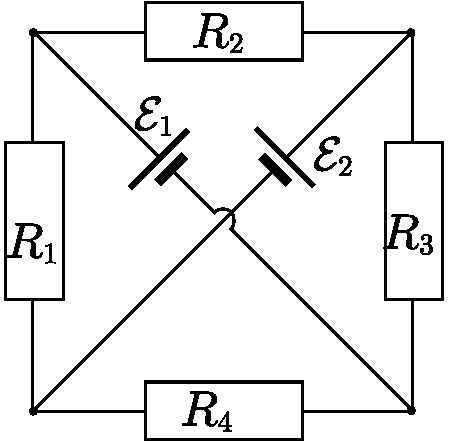
\includegraphics[width=0.35\linewidth]{2012-v3g-03-elektriline_sild}%
\end{center}
\fi


\ifHint
Peegelsümmeetria tõttu ülemises ja alumises takistis ($R_2$ ja $R_4$) vool puudub. 
\fi


\ifSolution
Sümmeetria tõttu ülemises ja alumises takistis ($R_2$ ja $R_4$) vool puudub. 
Tõepoolest, oletagem et ühes neist (nt $R_2$-s) läheb vool vasakult paremale. Peegeledame joonist vertikaaltelje
suhtes: $R_1$ ja $R_3$ ning ${\cal E}_1$ ja ${\cal E}_2$ vahetavad kohad, 
kuid takistite ning elektromotoorjõudude võrdsuse tõttu skeem ei muutu. Peegelduse käigus 
peaks nüüd vool muutma suuna vastupidiseks ning minema paremalt vasakule; esialgse ja 
peegelduse tulemusel saadud skeemi ekvivalentsuse tõttu peaks aga vool olema endiselt vasakult paremale,
mis viib vastuoluni. Järelikult on vool $R_2$-s ja $R_4$-s null ning skeemilt võib vastavad juhtmed kõrvaldada.
Järele jääb $R_1$, ${\cal E}_2$, $R_4$ ja ${\cal E}_2$ jadaühendus, mistõttu on voolutugevus ahelas, sh $R_1$-s ja $R_3$-s
leitav kui $I=2{\cal E}/2R = {\cal E}/R$.
\fi


\ifEngStatement
% Problem name: Whetstone bridge
In the circuit diagram given in the figure there are identical resistors with resistances $R_1 = R_2 = R_3 = R_4 = R$ and identical batteries with electromotive forces ${\cal E}_1 = {\cal E}_2
= {\cal E}$. Find the current strengths in the resistors (that means the expressions of $I_1$, $I_2$, $I_3$ and $I_4$ through the values of $R$ and ${\cal E}$).
\begin{center}
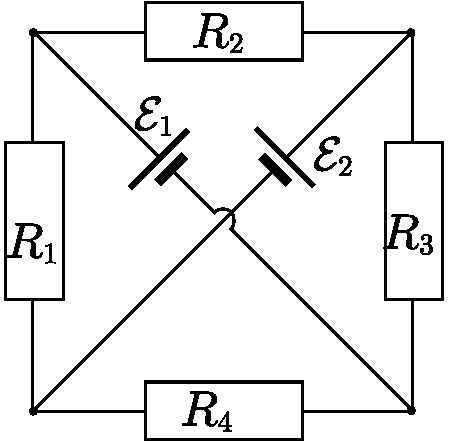
\includegraphics[width=0.35\linewidth]{2012-v3g-03-elektriline_sild}%
\end{center}
\fi


\ifEngHint
Because of mirror symmetry there is no current through the upper and the bottom resistor ($R_2$ and $R_4$).
\fi


\ifEngSolution
Due to symmetry in the upper and bottom resistor ($R_2$ and $R_4$) there is no current. Indeed, let us suppose that in one of them (for example in $R_2$) the current goes from left to right. We will reflect the figure with respect to the vertical axis: $R_1$ and $R_3$ as well as ${\cal E}_1$ and ${\cal E}_2$ will replace places, but due to the equality of the resistors and electromotive forces the diagram does not change. In the course of the reflection the current should now change the direction to the opposite and go from right to left; however, due to the initial diagram being equivalent to the diagram made with the reflection the current should still be from left to right which leads to a contradiction. Therefore the current in $R_2$ and $R_4$ is zero and the respective wires can be removed from the diagram. We are left with $R_1$, ${\cal E}_2$, $R_4$ and ${\cal E}_2$ that are connected in series, which is why the current in the diagram as well as in $R_1$ and $R_3$ can be found as $I=2{\cal E}/2R = {\cal E}/R$.
\fi
}